\documentclass{beamer}

% Theme
\usetheme{default}

% Title page
\title{Projet : CoreWar}
\author{Etienne BOSSU - Amand HENRY - Tom ROUSEE - Theo SICOT}
\date{\today}

% Slides
\begin{document}

\begin{frame}
    \titlepage
\end{frame}

\begin{frame}{Sommaire}
    \tableofcontents
\end{frame}

\begin{frame}{Introduction}
    \begin{itemize}
        \item But du projet : créer un jeu de CoreWar et un algorithme génétique permettant de créer des programmes efficaces avec Java.
        \vspace{\baselineskip}
        \item CoreWar : jeu de programmation où deux programmes s'affrontent dans une machine virtuelle (MARS).
    \end{itemize}
\end{frame}

\begin{frame}{Identification des objectifs :}
    Pour réaliser ce projet nous avons identifier plusieurs points clefs  du sujet:
    \vspace{\baselineskip}
    \begin{itemize}
        \item RedCode
        \item Machine MARS
        \item Algorithme génétique
        \item Interface graphique
    \end{itemize}
\end{frame}

\begin{frame}
    \frametitle{RedCode}
    Le RedCode :
    \begin{itemize}
        \item Langage de programmation type Assembleur
        \item Utilisé pour écrire les programmes des guerriers
        \item 11 instructions / 4 modes d'adressage
    \end{itemize}
\end{frame}

\begin{frame}
    \frametitle{MARS : Memory Array Redcode Simulator}
    C'est dans cette machine que les guerriers s'affrontent. Elle gère le déroulement de la partie, interprète le RedCode et gère la mémoire.
\end{frame}

\begin{frame}{Mémoire}
    \includegraphics[width=\textwidth]{img/umlMemoire.png}
\end{frame}

\begin{frame}{Le Déroulement d'une partie}
    
\end{frame}

\begin{frame}
    \frametitle{Interface graphique}
    Elle permet de visualiser le déroulement d'\textbf{une seule partie} de CoreWar.
    \begin{figure}
        \centering
        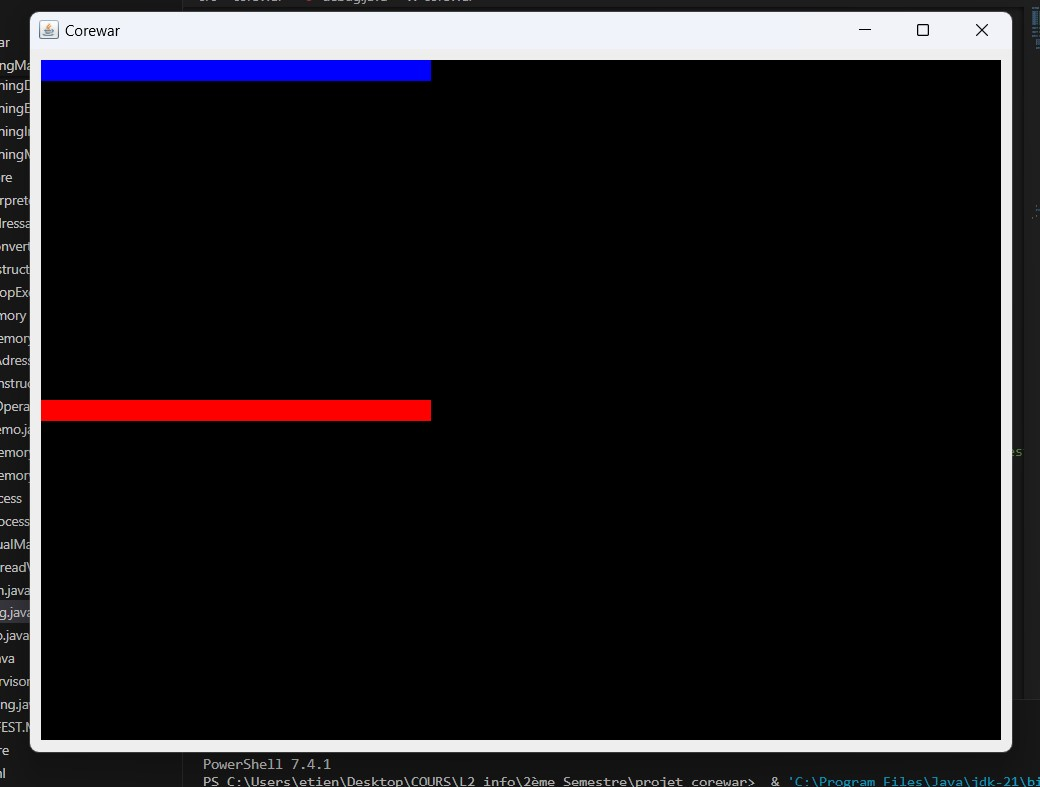
\includegraphics[width = 8cm]{img/display.jpg}
    \end{figure}
\end{frame}

\begin{frame}{Algorithme génétique}
    
\end{frame}

\begin{frame}{Fonctionnement de la reproduction}
    This is the main content slide.
\end{frame}

\begin{frame}{Algorithme génétique : Entrainement}
    This is the main content slide.
\end{frame}

\begin{frame}
    \frametitle{Résultats}
    Expliquer nos résultats
\end{frame}

\begin{frame}
    \frametitle{Conclusion}
    This is the conclusion slide.
\end{frame}

\begin{frame}{}
    \begin{center}
        \Huge Merci de votre attention
    \end{center}
\end{frame}

\end{document}